\documentclass[fleqn, 12pt]{article}
\usepackage[utf8]{inputenc} % default from sharelatex
\usepackage[a4paper, left=30mm, right=30mm, top=30mm, bottom=30mm]{geometry}
\usepackage{indentfirst} % to indent fist paragraph
\usepackage[brazilian]{babel} % BR
\usepackage{amsmath}
\usepackage{graphicx} % to have pictures

\graphicspath{{images/}}

\title{Teoria dos números e corpos finitos}

\author{Lucas João Martins}
\date{}

\begin{document}

\maketitle

\section*{}
\subsection*{1. (4.6) For each of the following equations, find an integer $x$
that satisfies the equation.}
  \subsubsection*{a. $5x \equiv 4 \ \ (mod \ \ 3)$}
    \begin{align*}
      & x = 2 \\
      & 5 \times 2 = 10 \\
      & 10 - 4 = 6 = 3 \times 2
    \end{align*}
  \subsubsection*{b. $7x \equiv 6 \ \ (mod \ \ 5)$}
    \begin{align*}
      & x = 3 \\
      & 7 \times 3 = 21 \\
      & 21 - 6 = 15 = 5 \times 3
    \end{align*}
  \subsubsection*{c. $9x \equiv 8 \ \ (mod \ \ 7)$}
    \begin{align*}
      & x = 4 \\
      & 9 \times 4 = 36 \\
      & 36 - 8 = 28 = 7 \times 4
    \end{align*}

\subsection*{2. (4.7) In this text, we assume that the modulus is a positive
integer. But the definition of the expression $a \ \ mod \ \ n$ also makes
 perfect sense if $n$ is negative. Determine the following:}

  Usando $a \ \ mod \ \ n = a - \lfloor a / n \rfloor \times n$.

  \subsubsection*{a. $5 \ \ mod \ \ 3$}
    \begin{align*}
      & 2
    \end{align*}
  \subsubsection*{b. $5 \ \ mod \ \ -3$}
    \begin{align*}
      & 5 - \lfloor 5 / -3 \rfloor \times -3 \\
      & 5 - (-2 \times -3) \\
      & 5 - 6 \\
      & -1 \\
    \end{align*}
  \subsubsection*{c.  $-5 \ \ mod \ \ 3$}
    \begin{align*}
      & -5 - \lfloor -5 / 3 \rfloor \times 3 \\
      & -5 - (-2 \times 3) \\
      & -5 + 6 \\
      & 1 \\
    \end{align*}
  \subsubsection*{d. $-5 \ \ mod \ \ -3$}
    \begin{align*}
      & -5 - \lfloor -5 / -3 \rfloor \times -3 \\
      & -5 - (1 \times -3) \\
      & -5 + 3 \\
      & -2 \\
    \end{align*}

\subsection*{3. (4.8) A modulus of 0 does not fit the definition but is defined
by convention as follows: $a \ \ mod \ \ 0 = a$. With this definition in mind,
what does the following expression mean: $a \equiv b \ \ (mod \ \ 0)$?}

  Significa que $a$ e $b$ são iguais.

\subsection*{4. (4.1) For the group $S_n$ of all permutations of $n$ distinct
symbols:}
  \subsubsection*{a. what is the number of elements in $S_n$?}

    $n!$

  \subsubsection*{b. show that $S_n$ is not abelian for $n > 2$.}

    Um contra exemplo com o $S_3$ seria:

    \begin{align*}
      & \lbrace 3, 2, 1 \rbrace \cdot \lbrace 1, 3, 2 \rbrace = \lbrace 2, 3, 1 \rbrace \\
      & \lbrace 1, 3, 2 \rbrace \cdot \lbrace 3, 2, 1 \rbrace = \lbrace 3, 1, 2 \rbrace \\
    \end{align*}

\subsection*{5. (4.4) Reformulate Equation (4.1), removing the restriction that
$a$ is a nonnegative integer. That is, let a be any integer.}

    A equação continua a mesma.

\subsection*{6. (4.5) Draw a figure similar to Figure 4.1 for $a < 0$.}
  \begin{figure}[h]
    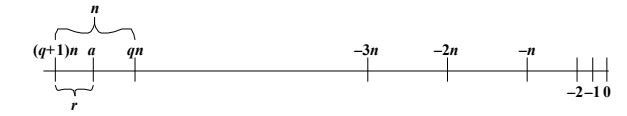
\includegraphics[width=\linewidth]{quatro_seis}
  \end{figure}

\subsection*{7. (4.13) Find the multiplicative inverse of each nonzero element in $Z_5$.}

    Para todo $a \in Z_5$, precisamos encontrar um $b \in Z_5$ onde $ab \equiv 1 \ \ (mod \ \ 5)$

    \begin{align*}
      & 1 \rightarrow 1 \\
      & 2 \rightarrow 3 \\
      & 3 \rightarrow 2 \\
      & 4 \rightarrow 4 \\
    \end{align*}

\subsection*{8. (4.20) Develop a set of tables similar to Table 4.3 for GF(5).}
  \begin{figure}[h]
    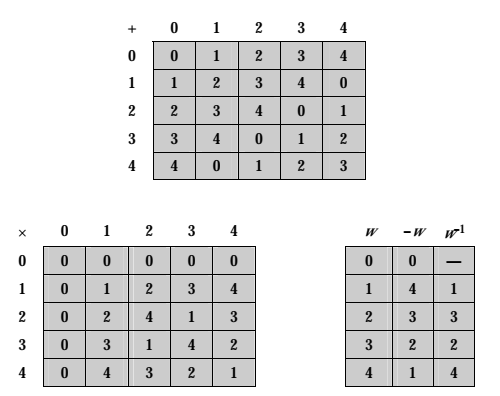
\includegraphics[width=\linewidth]{quatro_vinte}
  \end{figure}

\subsection*{9. (4.10) What is the smallest positive integer that has exactly k divisors, for $1 \leq k \leq 6$?}
  \begin{align*}
    & k = 1 \rightarrow 1 \rightarrow \lbrace 1 \rbrace \\
    & k = 2 \rightarrow 2 \rightarrow \lbrace 1, 2 \rbrace \\
    & k = 3 \rightarrow 4 \rightarrow \lbrace 1, 2, 4 \rbrace \\
    & k = 4 \rightarrow 6 \rightarrow \lbrace 1, 2, 3, 6 \rbrace \\
    & k = 5 \rightarrow 16 \rightarrow \lbrace 1, 2, 4, 8, 16 \rbrace \\
    & k = 6 \rightarrow 12 \rightarrow \lbrace 1, 2, 3, 4, 6, 12 \rbrace \\
  \end{align*}

\subsection*{10.}

\subsection*{11.}

\subsection*{12.}

\subsection*{13.}

\subsection*{14.}

\subsection*{15.}

\subsection*{16.}

\subsection*{17.}

\subsection*{18.}

\subsection*{19.}

\subsection*{20.}

\end{document}
